

    For all the examples we show here, we only show the ordering relations that are important to observe. 
    We exhaustively show for all the cases from Table \ref{reord:final_table} where reordering is not safe to do. 
    Some of these cases are addressed together as the same counter example suffices to show they are unsafe to do.

    \paragraph{Reads to same memory where $e$ is of type $sc$ and $d$ is either $uo/sc$}

        The following example illustrates when reordering two reads to $x$ as per the specification of their access orders and range results in an observable behavior disallowed.
        Figure~\ref{reord_counter:example1(a)} shows an example of a candidate (left) along with with its candidate execution (right) where the case of outcome in the red box is not possible. 
        \begin{figure}[H]
            \centering
            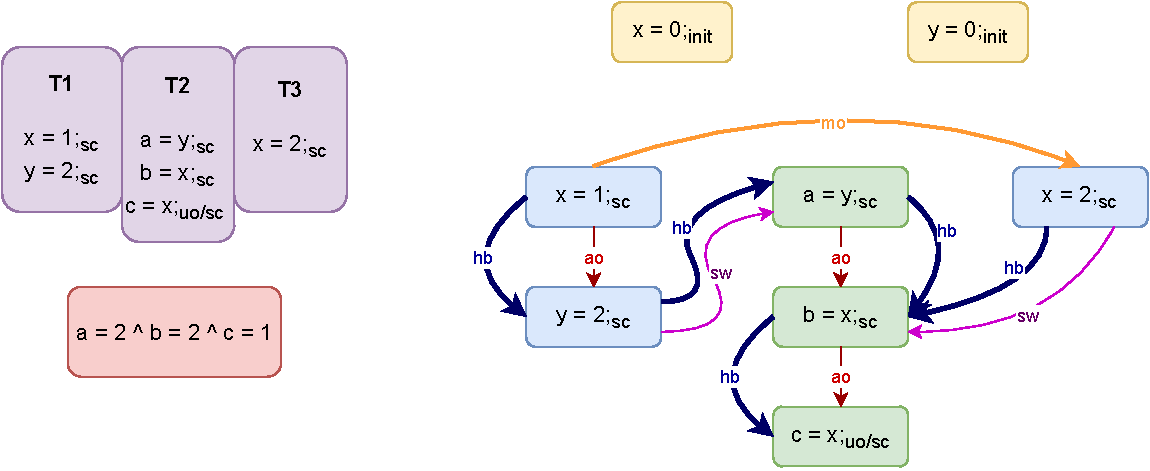
\includegraphics[scale=0.7]{7.CounterExamples/ReorderingCandidate/Example0(Rsc-Ruo,sc).pdf}
            \caption{Case where $a = 2, b = 2, c = 1$ is invalid due to Sequentially Consistent Atomics}
            \label{reord_counter:example1(a)}
        \end{figure}
        
        \begin{itemize}
            \item For $a=2$, it must come from the write $y=2;_{sc}$. 
            Thus, we would have $\reln{\{y=2;_{sc}\}}{sw}{\{a=y;_{sc}\}}$ and hence $\reln{\{y=2;_{sc}\}}{hb}{\{a=y;_{sc}\}}$.
            \item For $b=2$, it must come from the write $x=2$. 
            Thus, we would have $\reln{\{x=2;_{sc}\}}{sw}{\{b=x;_{sc}\}}$ and hence $\reln{\{x=2;_{sc}\}}{hb}{\{b=x;_{sc}\}}$.
            \item Using $\stck{_{ao}}$ and the above result, we can infer that $\reln{\{x=2;_{sc}\}}{mo}{\{x=2;_{sc}\}}$, $\reln{\{x=1;_{sc}\}}{hb}{\{c=x;_{uo/sc}\}}$ and $\reln{\{x=2;_{sc}\}}{hb}{\{c=x;_{uo/sc}\}}$.
            \item These relations correspond to patterns of Axiom \ref{SeqCsAt}, from which we can conclude that we cannot have $\reln{\{c=x;_{uo/sc}\}}{rf}{\{x=1;_{sc}\}}$.         
        \end{itemize}
        Hence, the observable behavior $a=2 \ \wedge \ b=2 \ \wedge \ c=1$ is disallowed.

        Figure~\ref{reord_counter:example1(b)} shows the Candidate (right) after reordering the two reads in $T2$ along with its candidate execution (left) where the same case of reads(orange box) is possible. 
        \begin{figure}[H]
            \centering
            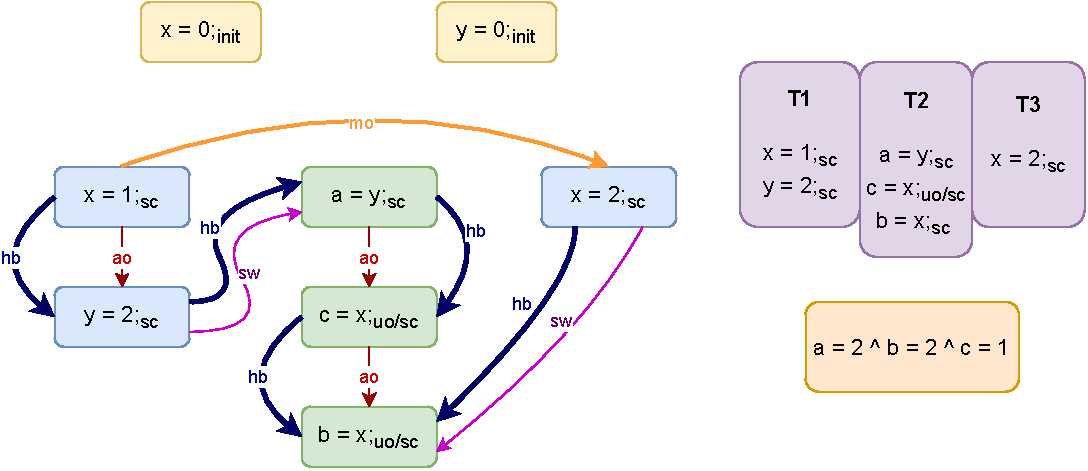
\includegraphics[scale=0.7]{7.CounterExamples/ReorderingCandidate/Example0R(Rsc-Ruo,sc).pdf}
            \caption{Case where the reads are reordered and $a = 2 , b = 2, c = 1$ is valid.}
            \label{reord_counter:example1(b)}
        \end{figure}

        \begin{itemize}
            \item For $a=2$, it must come from the write $y=2_{sc}$. 
            Thus, we would have $\reln{\{y=2;_{sc}\}}{sw}{\{a=y;_{sc}\}}$ and hence $\reln{\{y=2;_{sc}\}}{hb}{\{a=y;_{sc}\}}$.
            \item From this, we also get $\reln{\{x=1;_{sc}\}}{hb}{\{c=x;_{uo/sc}\}}$ and $\reln{\{x=1;_{sc}\}}{hb}{\{b=x;_{sc}\}}$.
            \item Now, for $c=1$, it must come from the write $\{x=1;_{sc}\}$. 
            This is possible as the above relations do not represent any pattern that restricts $\reln{\{c=x;_{uo/sc}\}}{rf}{\{x=1;_{sc}\}}$. .  
            \item Now for $b=2$, it must come from the write $\{x=2;_{sc}\}$.
            Since there is no happens-before or memory-order relations with this write, none of the axioms would restrict $\reln{\{b=x;_{sc}\}}{rf}{\{x=2;_{sc}\}}$.        
        \end{itemize}
        Thus, the observable behavior $a=1 \ \wedge \ b=2 \ \wedge \ c=2$ is allowed by the program after reordering. 
        
%---------------------------------------------------------------------------------------------------------------------------------------
    
    \paragraph{A Read $e$ of type $sc$ followed by a Write of either $uo/sc$}
        
        Figure~\ref{reord_counter:example2(a)} shows an example of a candidate (left) along with with its candidate execution (right) where the case of outcome in the red box is not possible. 
        \begin{figure}[H]
            \centering
            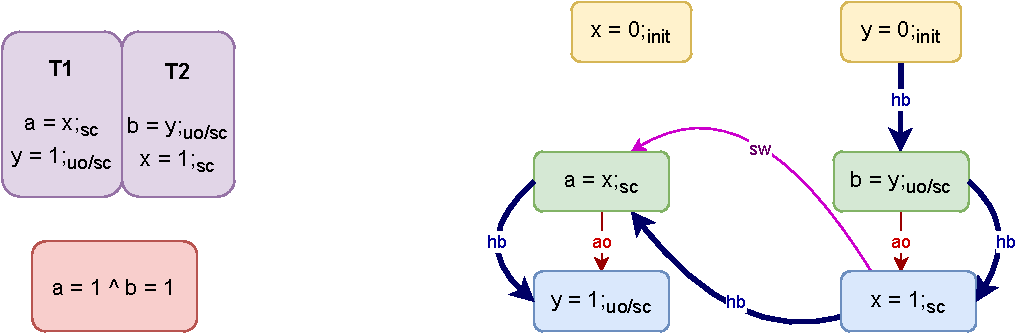
\includegraphics[scale=0.7]{7.CounterExamples/ReorderingCandidate/Example3(Rsc-Wuo,sc).pdf}
            \caption{Case where $a = 1, b = 1$ is invalid due to Coherent Reads.}
            \label{reord_counter:example2(a)}
        \end{figure}

        Observations:
        \begin{itemize}
            \item For $a=1$, it must come from the write $x=1_{sc}$. 
            Thus, we would have $\reln{\{x=1;_{sc}\}}{sw}{\{a=x;_{sc}\}}$ and hence $\reln{\{x=1;_{sc}\}}{hb}{\{a=x;_{sc}\}}$.
            \item From the above relation and using $\stck{_{ao}}$, we can infer $\reln{\{b=y_{uo/sc}\}}{hb}{\{y=1_{uo/sc}\}}$
            \item The above relation corresponds to a pattern of Axiom \ref{CoRe}, from which we can infer that we cannot have the relation  $\reln{\{b=y;_{uo/sc}\}}{rf}{\{y=1;_{uo/sc}\}}$.        
        \end{itemize}
        Hence, the observable behavior $a=1 \ \wedge \ b=1$ is disallowed.

        Figure~\ref{reord_counter:example2(b)} shows the Candidate after reordering(right) a read and write in $T1$ along with its candidate execution(left) where the same case of reads(orange box) is possible. 
        \begin{figure}[H]
            \centering
            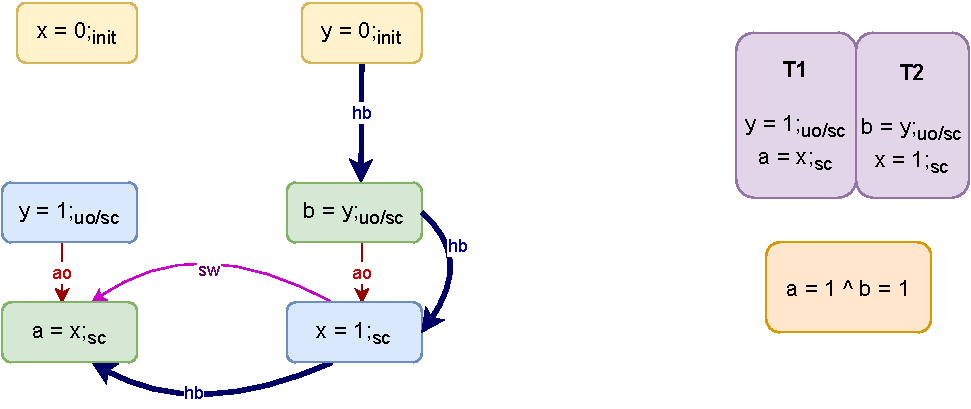
\includegraphics[scale=0.7]{7.CounterExamples/ReorderingCandidate/Example3R(Rsc-Wuo,sc).pdf}
            \caption{Case where events of T1 are reordered, resulting in $a = 1, b = 1$ to be valid.}
            \label{reord_counter:example2(b)}
        \end{figure}
        
        Observations:
        \begin{itemize}
            \item For $a=1$, it must come from the write $x=1_{sc}$. 
            Thus, we would have $\reln{\{x=1;_{sc}\}}{sw}{\{a=x;_{sc}\}}$ and hence $\reln{\{x=1;_{sc}\}}{hb}{\{a=x;_{sc}\}}$.
            \item From the above, we cannot infer $\reln{\{b=y_{uo/sc}\}}{hb}{\{y=1_{uo/sc}\}}$. In fact no happens-before relation can exist between the two events.
            \item We can have the relation $\reln{\{b=y;_{uo/sc}\}}{rf}{\{y=1;_{uo/sc}\}}$.
        \end{itemize}
        Hence, the observable behavior $a=1 \ \wedge \ b=1$ is allowed.
%--------------------------------------------------------------------------------------------------------------------------------------        
    \paragraph{A Read $e$ of type $uo$ followed by a write $d$ of type $sc$}

        For this we can use the same example in Figure~\ref{reord_counter:example2(a)} where we just reorder $T2$'s events.
        We leave justifying the new observable behavior introduced as an exercise for the reader.
    
%---------------------------------------------------------------------------------------------------------------------------------------
        
    \paragraph{A Write $e$ followed by a Read $d$ both of type $sc$}
        
        A counter example for this is different. 
        It is not the Observable Behavior we are concerned with that is introduced, but that which is allowed after reordering creates a $\stck{_{hb}}$ cycle. 
        Figure~\ref{reord_counter:example3(a)} is one such example with its Candidate and Corresponding Candidate Execution in question:
        \begin{figure}[H]
            \centering
            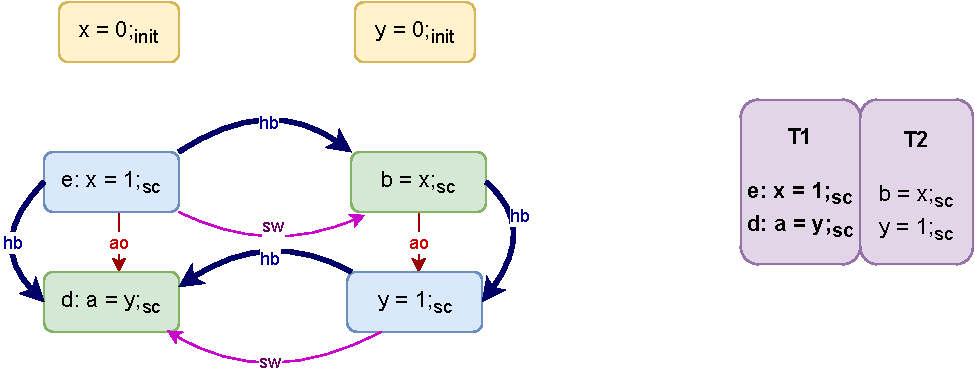
\includegraphics[scale=0.7]{7.CounterExamples/ReorderingCandidate/Example5(Wsc-Rsc).pdf}
            \caption{Case where $a = 1, b = 1$ is valid and no happens-before cycles}
            \label{reord_counter:example3(a)}
        \end{figure}

        Figure~\ref{reord_counter:example3(b)} shows the Candidate after reordering(right) the two events in $T1$, which makes the same candidate execution(right) as above contain a happens-before cycle:
        \begin{figure}[H]
            \centering
            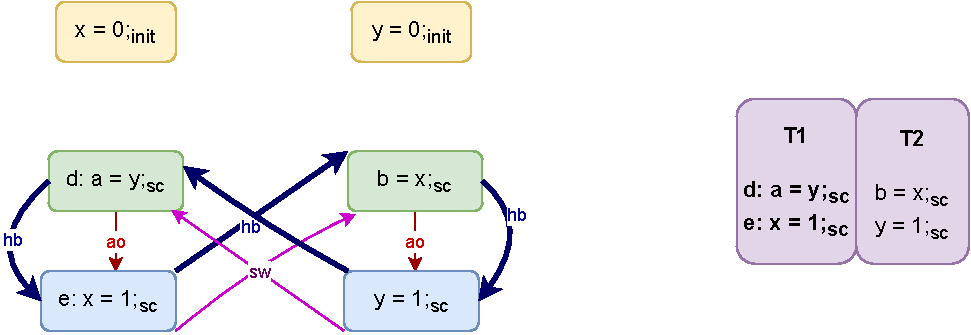
\includegraphics[scale=0.7]{7.CounterExamples/ReorderingCandidate/Example5R(Wsc-Rsc).pdf}
            \caption{Case where $a = 1, b = 1$ implies a happens-before cycle}
            \label{reord_counter:example3(b)}
        \end{figure}

        Observation:
        \begin{itemize}
            \item From the read values we can infer that the Candidate Execution should have $\reln{\{x=1_{sc}\}}{hb}{\{a=x_{sc}\}}$ and $\reln{\{y=1_{sc}\}}{hb}{\{a=y_{sc}\}}$.
            \item The above relations create the cycle $\reln{\{a=y_{sc}\}}{hb}{\reln{\{x=1_{sc}\}}{hb}{\reln{\{a=x_{sc}\}}{hb}{\reln{\{y=1_{sc}\}}{hb}{\{a=y_{sc}\}}}}}$.
            \item This execution is invalid. 
        \end{itemize}

        One might think that simply discarding the above Candidate execution would do. 
        But this would mean discarding certain $\stck{_{hb}}$ relations by considering them to be irrelevant; this would require more information to infer which relations are going to create such cycles and which are not. 
        In practice a cycle may span several events from different threads.
        Since we place no assumptions on these relations.
        Hence, the following reordered program outcome is something we do not risk to allow.

%---------------------------------------------------------------------------------------------------------------------------------------

    \paragraph{A Write $e$ of type $uo/sc$ followed by a Write $d$ of type $sc$}
        
        Figure~\ref{reord_counter:example4(a)} shows an example of a candidate(left) along with with its candidate execution(right) where the case of outcome in the red box is not possible. 
        \begin{figure}[H]
            \centering
            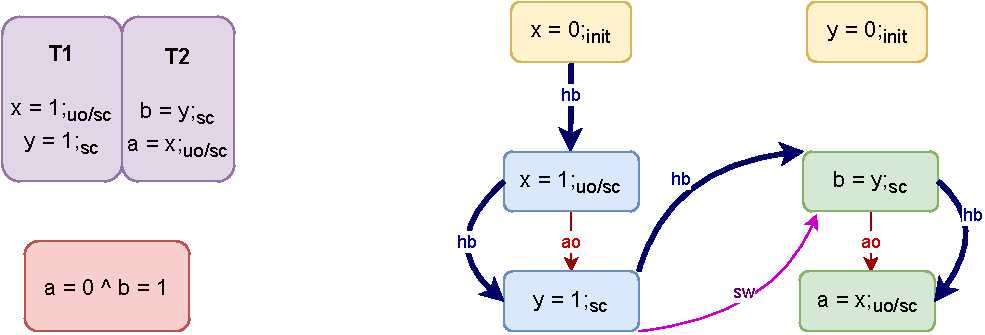
\includegraphics[scale=0.7]{7.CounterExamples/ReorderingCandidate/Example7(Wuo,sc-Wsc).pdf}
            \caption{Case where $a = 0, b = 1$ is invalid due to Coherent Reads.}
            \label{reord_counter:example4(a)}
        \end{figure}
        
        Observations:
        \begin{itemize}
            \item For $b=1$, it must come from the write $y=1_{sc}$. 
            Thus, we would have $\reln{\{y=1;_{sc}\}}{sw}{\{b=y;_{sc}\}}$ and hence $\reln{\{y=1;_{sc}\}}{hb}{\{b=y;_{sc}\}}$.
            \item From the above relation, we can infer $\reln{\{x=0_{init}\}}{hb}{\reln{\{x=1_{uo/sc}\}}{hb}{\{a=x_{uo/sc}\}}}$.
            \item The above relation corresponds to a pattern of Axiom \ref{CoRe}, from which we can conclude that we cannot have $\reln{\{a=x;_{uo/sc}\}}{rf}{\{x=0;_{init}\}}$.
        \end{itemize}
        Hence, the observable behavior $a=0 \ \wedge \ b=1$ is disallowed.

        Figure~\ref{reord_counter:example4(b)} shows the Candidate after reordering(right) the two writes in $T1$ along with its candidate execution(left) where the same case of reads(orange box) is possible. 
        \begin{figure}[H]
            \centering
            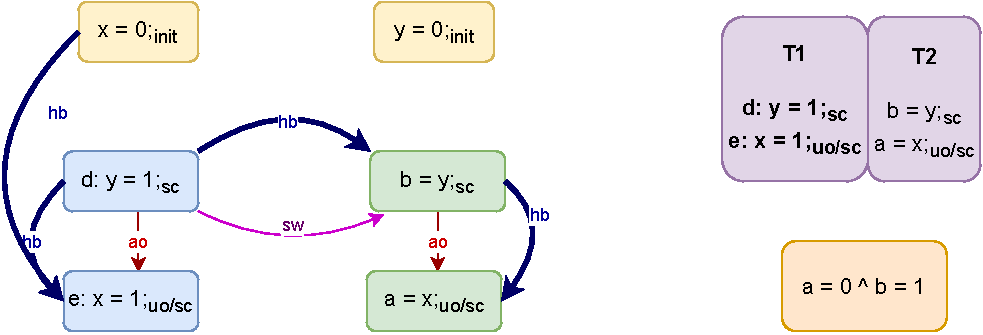
\includegraphics[scale=0.7]{7.CounterExamples/ReorderingCandidate/Example7R(Wuo,sc-Wsc).pdf}
            \caption{Case where events of T1 are reordered, resulting in $a = 0,  b = 1$ to be valid.}
            \label{reord_counter:example4(b)}
        \end{figure}
        
        Observations:
        \begin{itemize}
            \item For $b=1$, it must come from the write $y=1_{sc}$. 
            Thus, we would have $\reln{\{y=1;_{sc}\}}{sw}{\{b=y;_{sc}\}}$ and hence $\reln{\{y=1;_{sc}\}}{hb}{\{b=y;_{sc}\}}$.
            \item From the above relation and $\stck{_{ao}}$, we cannot infer $\reln{\{x=1_{uo/sc}\}}{hb}{\{a=x_{uo/sc}\}}$.
            \item Thus, we can have  $\reln{\{a=x;_{uo/sc}\}}{rf}{\{x=0;_{init}\}}$.
        \end{itemize}
        Hence, the observable behavior $a=0 \ \wedge \ b=1$ is allowed.